\documentclass[a4paper,12pt]{article}
\usepackage[UTF8]{ctex}
\usepackage{tocloft}
\usepackage{graphicx}
\usepackage{caption}
\usepackage{hyperref}
%定义图片位置
\graphicspath{{./Figure}}
%重定义图注
\captionsetup[figure]{name=Figure, labelsep=colon}
% 重定义目录命令,以居中显示目录标题
\renewcommand{\contentsname}{\hfill\bfseries\Large 目录\hfill}   
\renewcommand{\cftaftertoctitle}{\hfill}

%调整红框
\hypersetup{
    colorlinks=false,% 使用边框而不是颜色链接
    pdfborderstyle={/S/U/W 0} % 无边框
}

% 定义一个用于图表引用的命令,仅为引用添加红色边框
\newcommand{\figref}[1]{%
    \begingroup
    \hypersetup{pdfborderstyle={/S/S/W 1}, linkbordercolor={1 0 0}} % 方框样式,红色
    \ref{#1}%
    \endgroup
}

\begin{document}
% 更改封面的字体样式
\title{\huge My Test Document}
\author{{\large knight-zzm}}
\date{\today}
\maketitle
\thispagestyle{empty} % 封面页无页码
\newpage

\tableofcontents
\thispagestyle{empty} % 无页码
\newpage
\pagenumbering{arabic}
\section{练习latex 论文写作}
This is the introduction.

\subsection{图表的创建和引用}
    The above data is combined to form a correlation heat map bettween features,as show in Fig.\figref{fig:time-freq}
    \begin{figure}[h]
        \centering
        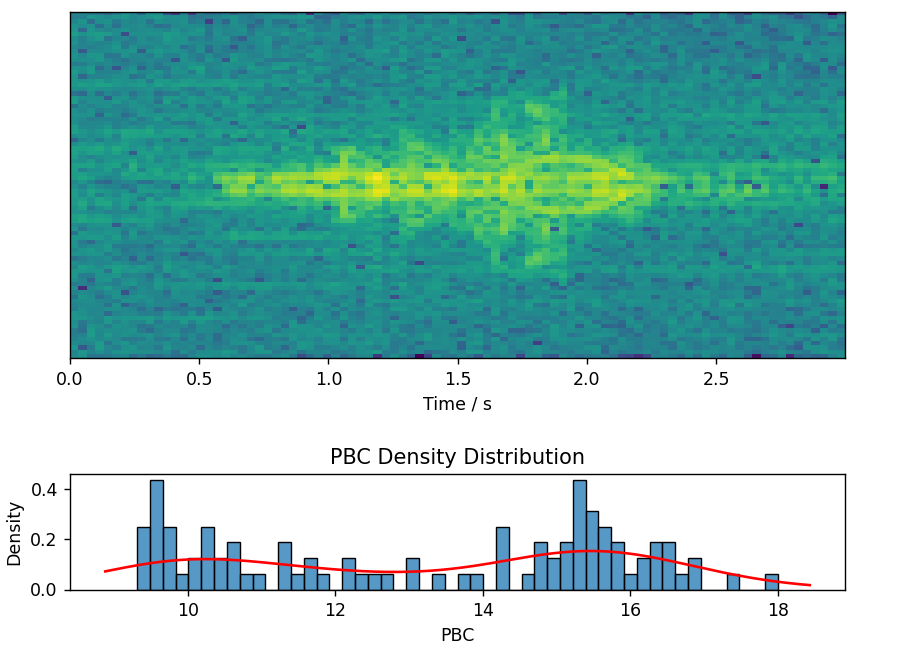
\includegraphics[width=1\textwidth]{时频图和PBC分布图.png}
        \caption{时频图和PBC分布图}
        \label{fig:time-freq}
    \end{figure}

\subsection{公式编辑和引用}
    1.太阳高度角 
    $$
\begin{aligned}
& \alpha_s \text { [3] } \\
& \gamma_s \text { [4] } \\
& \sin \alpha_s=\cos \delta \cos \varphi \cos \omega+\sin \delta \sin \varphi \\
& \cos \gamma_s=\frac{\sin \delta-\sin \alpha_s \sin \varphi}{\cos \alpha_s \cos \varphi}
\end{aligned}
$$


\subsection{表格编辑和引用}
    \begin{tabular}{|c|c|c|c|}
        \hline
        \multicolumn{2}{|c|}{MCM} & \multicolumn{2}{|c|}{ICM} \\
        \hline
        A & 连续型 & D & 运筹学/网络科学\\
        \hline
        B & 离散型 & E & 环境科学\\
        \hline
        C & 大数据 & F & 政策\\
        \hline
    \end{tabular}
    
    \begin{tabular}{rc}
    Apples & Green\\
    \hline 
    Strawberries & Red \\
    \cline{1-1}
    Oranges & Orange \\
    \end{tabular}
    
    \begin{tabular}{|r|l|}
    \hline
    8 & here's \\
    \cline{2-2}
    86 & stuff\\
    \hline \hline 
    2008 & now \\
    \hline 
    \end{tabular}

\end{document}

